\documentclass[a4paper,11pt]{report}
\usepackage{polski}
\usepackage[utf8]{inputenc}
\usepackage{graphicx} % obrazki
\usepackage{fancyvrb} % spacje w verbatim
\usepackage[table]{xcolor}
\usepackage{geometry}
\usepackage{indentfirst}
\usepackage{arydshln}
\usepackage{tikz}
\usepackage{amsmath}
\usepackage{pgfplots}
\pgfplotsset{every tick label/.append style={font=\footnotesize}}
\title{Quicksort}
\author{Rafał Stępień Krzysztof Kotlarz}
\date{\today}
\begin{document}
\renewcommand{\tabcolsep}{10mm}
\newgeometry{tmargin=2cm,bmargin=2cm,lmargin=2cm,rmargin=2cm}

\begin{titlepage}
   \begin{center}
       \vspace*{9cm}
 
       \textbf{\huge{Quicksort - sortowanie szybkie}}
 
       \vspace{1.5cm}
 
       Rafał Stępień | Krzysztof Kotlarz \\
       \vspace{2cm}

 
       Wydział Biologii i Hodowli Zwierząt\\
       Uniwersytet Przyrodniczy we Wrocławiu\\
       Bioinformatyka\\
 
   \end{center}
\end{titlepage}
\newpage
\tableofcontents
\begin{abstract}
Quicksort został wynaleziony przez brytyjskiego informatyka Tony'ego Hoare'a. Jest jednym z najpopularniejszych algorytmów sortujących. Do dnia dzisiejszego jest powszechnie używany, jednak ze względu na rekurencyjne działanie, trzeba uważać przy jego stosowaniu i nie można go implementować bezmyślnie. Stosowanie go bez wymaganej wiedzy może prowadzić to do przepełnienia stosu rekurencji i zablokowania komputera, lub spadku wydajności.



W przypadku rozważania efektywności algorytmu quicksort bierze się pod uwagę przede wszystkim dwa przypadki: najlepszy i średni, można jednak wysnuć intuicje dotyczące przypadku najgorszego. Wydajność algorytmu będzie zależna miedzy innymi od stopnia posortowania listy jak i metody wyboru \textit{pivot'}a
\end{abstract}

\chapter{Quicksort}
\section{Zasada działania}
Algorytm jest oparty na technice "dziel i zwyciężaj", którą możemy podzielić na 3 kroki:
\begin{enumerate}
\item \textbf{Dziel} - Tablica $A[]$ jest dzielona na dwie części, takie, że każdy element tablicy pierwszej jest nie większy niż $A[q]$, a każdy element tablicy drugiej jest większy od $A[q]$. Możemy wywnioskować że bardzo ważnym krokiem będzie wybór elementu $A[q]$.
\item \textbf{Zwyciężaj} - Obydwie podtablice są sortowane rekurencyjnymi wywołaniami quicksort.
\item \textbf{Połącz} - Z racji tego, że sortowanie odbywa się w miejscu nie musimy łączyć tablic, ponieważ są one już automatycznie połączone.
\end{enumerate}
\subsection*{Właściwości algorytmu}
\begin{itemize}
\item \textbf{Sortowanie w miejscu} - zaletą takiego działania jest to, że nie zużywamy dodatkowej pamięci, ponieważ operacje są wykonywane za każdym razem na tej samej liście, nie tworzymy nowej.
\item \textbf{Szybkość średniego przypadku} - jego oczekiwany czas działania wynosi $\theta(nlgn)$, a stałe ukryte pod znakiem $\theta$ są małe.
\item Działa dobrze w środowiskach wykorzystujących \textbf{pamięć wirtualną}
\end{itemize}
\newpage
\section{Podział tablicy}
Dzięki funkcji def partition następuje podzielenie większych problemów na mniejsze. Wykorzystany zostanie pivot, czyli element który pozwoli wyznaczyć na dwa podproblmy. Elementy na lewo od pivot'a będą od niego mniejsze, zaś po jego prawej stronie, większe.


Procedurę zaczęto od wybrania wartości \textit{p}, która ma być pivotem wg. jednej z 4 funkcji (wartość ze zbioru znajdująca się na: końcu, początku, w miejscu środkowym lub z losowego miejsca), względem której będzie dokonywany podział. Indeksem pivota zawsze zostaje miejsce będące ostatnią pozycją analizowanego przedziału.


Element $i$-ty to element obecnie poddawany analizie w ciele pętli. natomiast element $j$-ty jest to tzw. border 
w którego miejsce wstawiane będą elementy $i$-te. Ostatecznie border wyznacza miejsce w które trafić ma pivot po wyjściu z pętli oraz miejsce zawierające element posortowany, który znajduje się we właściwym miejscu. Pivot nie zostaje analizowany podczas iteracji


Procedurę zaczynamy zawsze od początku do końca wyznaczonego zbioru. Element $i$-ty zostaje zamieniony z $j$-tym w momencie, gdy i$<$p. Zbiór analizowany jest element po elemencie. Gdy następuje zamiana, element $j$ zostaje przesunięty $+1$. Komórki zaznaczone na szaro to elementy ulegające zamianie w danej iteracji.
\begin{table}[h!]
\Large
\centering
\begin{tabular}{|c|c|c|c|c|c|}
\hline
\cellcolor{black!25} &  &  &  &  & \\
\cellcolor{black!25}2 & 8 & 7 & 1 & 3 & 5 \\ \hdashline
i=j&  & &  &  & p\\ \hline
\end{tabular}

\end{table}

Element $i$-ty = 2 jest mniejszy od p$=$5. Zostaje on zamieniony z elementem $j$-tym. W tym przypadku następują zamiana w miejscu.

\begin{table}[h!]
\Large
\centering
\begin{tabular}{|c|c|c|c|c|c|}
\hline
 &  &  &  &  & \\
2 & 8 & 7 & 1 & 3 & 5 \\ \hdashline
 & i=j & &  &  & p\\ \hline
\end{tabular}

\end{table}

Po zamianie następuje przesunięcie elementu $j$-tego +1. Rozpoczęto analizę kolejnego $i$-tego elementu.

\begin{table}[h!]
\Large
\centering
\begin{tabular}{|c|c|c|c|c|c|}
\hline
 &  &  &  &  & \\
2 & 8 & 7 & 1 & 3 & 5 \\ \hdashline
 & j & i &  &  & p\\ \hline
\end{tabular}

\end{table}

\begin{table}[h!]
\Large
\centering
\begin{tabular}{|c|c|c|c|c|c|}
\hline
 & \cellcolor{black!25} &  & \cellcolor{black!25} &  & \\
2 & \cellcolor{black!25}8 & 7 & \cellcolor{black!25}1 & 3 & 5 \\ \hdashline
 & j &   & i &  & p\\ \hline
\end{tabular}

\end{table}

Elementy i$=$1 jest mniejszy od wartości $p=$5 zostaje zamieniony z elementem $j=$8


\begin{table}[h!]
\Large
\centering
\begin{tabular}{|c|c|c|c|c|c|}
\hline
 &  &\cellcolor{black!25}  &  & \cellcolor{black!25} & \\
2 & 1 & \cellcolor{black!25}7 & 8 & \cellcolor{black!25}3 & 5 \\ \hdashline
 &   & j  &   & i & p\\ \hline
\end{tabular}

\end{table}

Elementy i$=$3 jest mniejszy od wartości p$=$5 zostaje zamieniony z elementem $j=$7 

\begin{table}[h!]
\Large
\centering
\begin{tabular}{|c|c|c|c|c|c|}
\hline
 &  &  & \cellcolor{black!25} &  &\cellcolor{black!25} \\
2 & 1 & 3 & \cellcolor{black!25}8 & 7 &\cellcolor{black!25} 5 \\ \hdashline
 &   &   & j  &  & p\\ \hline
\end{tabular}

\end{table}

Pivot nie jest analizowany w pętli. Gdy pętla dobiegnie końca pivot $p$ zamieniany jest z elementem $j-$tym.


\begin{table}[h!]
\Large
\centering
\begin{tabular}{|c|c|c|c|c|c|}
\hline
\multicolumn{3}{|c|}{Lewa część tablicy} & Pivot & \multicolumn{2}{c|}{Prawa część tablicy} \\ \hline
2 & 1 & 3 & \textbf{5} & 7 & 8 \\ \hdashline
 &  &  &  &  &  \\ \hline
\end{tabular}

\end{table}

Duży problem został podzielony na dwa mniejsze; lewą oraz prawą część tablicy. W momencie pivot $p$ jest uważany za posortowany, który znajduje się we właściwym dla siebie miejscu. Następnie rekurencyjnie wywołujemy tą samą funkcje, jednak tym razem dotyczyć ona będzie jedynie jednego z podproblemów. Funkcja $partition$ analizować będzie teraz lewą część tablicy

\begin{table}[h!]
\Large
\centering
\begin{tabular}{|c|c|c|}
\hline
\multicolumn{3}{|c|}{Lewa część tablicy} \\ \hline
\cellcolor{black!25}2 & 1 & 3 \\ \hdashline
i=j &  & p \\ \hline
\end{tabular}

\end{table}

Procedura jest identyczna jak w przypadku pierwszego wykonania funkcji. Pozycja pivota $p$ znajduje się na ostatniej pozycji analizowanego zbioru. Iteracje rozpoczynamy od początku listy. 


Elementy $i=$2 jest mniejszy od wartości $p=$3 zostaje on zamieniony z elementem $j=$2. W tym przypadku następuje zamiana w miejscu.


\begin{table}[h!]
\Large
\centering
\begin{tabular}{|c|c|c|}
\hline
 & \cellcolor{black!25} &   \\
2 & \cellcolor{black!25}1 & 3 \\ \hdashline
 & i=j  & p \\ \hline
\end{tabular}

\end{table}

Po zamianie następuje przesunięcie elementu j-tego +1. Rozpoczęto analize kolejnego i-tego elementu. Elementy $i=$1 jest mniejszy od wartości $p=$3 zostaje on zamieniony z elementem $j=$1. W tym przypadku następuje zamiana w miejscu.


\begin{table}[h!]
\Large
\centering
\begin{tabular}{|c|c|c|}
\hline
 &  & \cellcolor{black!25}  \\
2 & 1 & \cellcolor{black!25}3 \\ \hdashline
 &   & j=p \\ \hline
\end{tabular}

\end{table}

Pivot nie jest analizowany w pętli. Gdy pętla dobiegnie końca pivot $p$ zamieniany jest z elementem $j$-tym.

\begin{table}[h!]
\Large
\centering
\begin{tabular}{|c|c|c|}
\hline
\multicolumn{2}{|c|}{Lewa część tablicy} & Pivot \\ \hline
2 & 1 & \textbf{3}\\ \hdashline
 &  &  \\ \hline
\end{tabular}
\end{table}

Pivot $p$ znajduje się we właściwym dla siebie miejscu. 
Następuje analiza kolejnego podproblemu. Zbiór składa się z lewej części tablicy zawierającej 2 elementy, oraz prawej części tablicy zawierającej 0 elementów.

\begin{table}[h!]
\Large
\centering
\begin{tabular}{|c|c|}
\hline
\multicolumn{2}{|c|}{Lewa część} \\ \hline
\cellcolor{black!25}2 & 1 \\ \hdashline
i=j & p \\ \hline
\end{tabular}

\end{table}


\begin{table}[h!]
\Large
\centering
\begin{tabular}{|c|c|}
\hline
\cellcolor{black!25} &  \cellcolor{black!25}\\ 
\cellcolor{black!25}2 & \cellcolor{black!25}1 \\ \hdashline
j & p \\ \hline
\end{tabular}

\end{table}

Pozycja pivota $p$ znajduje się na ostatniej pozycji analizowanego zbioru. Iteracje rozpoczynamy od początku listy. 


Element $i=$2 nie zostaje przeniesiony. Pivot $p$ nie jest analizowany, zamieniany jest z elementem $j$-tym.

\begin{table}[h!]
\Large
\centering
\begin{tabular}{|c|c|}
\hline
 Lewa część & Pivot \\ \hline
1 &  \textbf{2}\\ \hdashline
 &  \\ \hline
\end{tabular}
\end{table}


Pivot $p$ znajduje się we właściwym dla siebie miejscu.

\begin{table}[h!]
\Large
\centering
\begin{tabular}{|c|}
\hline
Lewa \\ \hline
\textbf{1} \\ \hdashline
 \\ \hline
\end{tabular}

\end{table}

Ze względu na warunek rekurencji $start < stop$ część jednoelementowa nie podlega analizie. Element znajduje się we właściwej dla siebie pozycji.

\begin{table}[h!]
\Large
\centering
\begin{tabular}{|c|c|c|c|c|c|}
\hline
\multicolumn{3}{|c|}{Lewa część tablicy} & Pivot & \multicolumn{2}{c|}{Prawa część tablicy} \\ \hline
2 & 1 & 3 & \textbf{5} & 7 & 8 \\ \hdashline
 &  &  &  &  &  \\ \hline
\end{tabular}

\end{table}

Kolejne wywołanie rekurencyjne będzie analizowało prawą część tablicy.


\begin{table}[h!]
\Large
\centering
\begin{tabular}{|c|c|}
\hline
\multicolumn{2}{|c|}{Prawa część} \\ \hline
\cellcolor{black!25}7 & 8 \\ \hdashline
i=j & p \\ \hline
\end{tabular}

\end{table}

Elementy $i=$7 jest mniejszy od wartości $p=$8 zostaje on zamieniony z elementem $j=$7. Następuje zamiana w miejscu.


\begin{table}[h!]
\Large
\centering
\begin{tabular}{|c|c|}
\hline
 &  \cellcolor{black!25}\\ 
7 & \cellcolor{black!25}8 \\ \hdashline
 & j=p \\ \hline
\end{tabular}

\end{table}
Po zamianie następuje przesunięcie elementu $j$-tego +1. Pivot $p$ zamieniany jest z elementem $j$-tym. Następuje zamiana w miejscu

\begin{table}[h!]
\Large
\centering
\begin{tabular}{|c|c|}
\hline
 Lewa część & Pivot \\ \hline
7 &  \textbf{8}\\ \hdashline
 &  \\ \hline
\end{tabular}

\end{table}

Pivot $p$ znajduje się we właściwym dla siebie miejscu. 

\begin{table}[h!]
\Large
\centering
\begin{tabular}{|c|}
\hline
Lewa \\ \hline
\textbf{7} \\ \hdashline
 \\ \hline
\end{tabular}

\end{table}

Pivot $p$ znajduje się we właściwym dla siebie miejscu. Ze względu na warunek rekurencji część jednoelementowa nie podlega analizie. Element znajduje się we właściwej dla sienie pozycji.


Po "sprasowaniu" wszystkich elementów \textbf{pogrubionych} otrzymamy posortowaną listę.

\subsection{Implementacja w Python}

\begin{verbatim}
def partition(lst, start, stop):
    pivot_index = stop
    pivot_value = lst[pivot_index]
    for i in range(start, stop):
        if lst[i] < pivot_value:
            lst[i], lst[start] = lst[start], lst[i]
            start += 1
    lst[stop], lst[start] = lst[start], lst[stop]
    return start
\end{verbatim}


\section{Wybór pivot'a}
Pivot można ustalać na 4 różne sposoby. Są to kolejno:
\begin{itemize}
\item ostatni element na analizowanej liście,
\item pierwszy element na analizowanej liście, 
\item element o środkowym indeksie
\item element losowo wybrany z analizowanej listy
\end{itemize} 
Wszystkie te podejścia testujemy w naszym kodzie.

\subsection{Implementacja w Python}

\begin{verbatim}
def partition_last(lst, start, stop):
    lst[stop], lst[stop] = lst[stop], lst[stop]
    return partition(lst, start, stop)
\end{verbatim}
\textbf{Partition last} - pivot wybierany jako ostatni element z analizowanej listy.

\begin{verbatim}
def partition_rand(lst, start, stop):
    rand_pivot = random.randint(start, stop)
    lst[stop], lst[rand_pivot] = lst[rand_pivot], lst[stop]
    return partition(lst, start, stop)
\end{verbatim}
\textbf{Partition rand} - pivot wybierany jako losowy element z analizowanej listy.

\begin{verbatim}
def partition_first(lst, start, stop):
    lst[stop], lst[start] = lst[start], lst[stop]
    return partition(lst, start, stop)
\end{verbatim}
\textbf{Partition last} - pivot wybierany jako pierwszy element z analizowanej listy.

\begin{verbatim}
def partition_middle(lst, start, stop):
    med = (len(lst)) // 2
    lst[stop], lst[med] = lst[med], lst[stop]
    return partition(lst, start, stop)
\end{verbatim}
\textbf{Partition last} - pivot wybierany jako środkowy element z analizowanej listy.

\section{Funkcja właściwa \textit{Quicksort}}

Jeśli długość tablicy jest większa niż indeks pierwszego elementu, to do zmiennej q zapisz wynik procedury "partition" na podanej tablicy A (czyli indeks pivota), i dokonaj podziału dwóch utworzonych podtablic metodą quicksort: 

\begin{verbatim}
def quick_sort(lst, start, stop, fun):
    if start < stop:
        border = fun(lst, start, stop)
        quick_sort(lst, start, border - 1, fun)
        quick_sort(lst, border + 1, stop, fun)
\end{verbatim}

Definiujemy funkcję quicksort, przyjmującą parametry:

\begin{itemize}
\item \textit{lst} - lista, przekazana do sortowania
\item \textit{start} - punkt początkowy (start iteracji)
\item \textit{stop} - punkt końcowy (koniec iteracji)
\item \textit{fun} - funkcja wyboru pivot'a (wybierana spośród czterech: element pierwszy, ostatni, losowy, lub o środkowym indeksie z analizowanego podzbioru.
\end{itemize}

Blok \textit{if} warunkuje, że ostatni element na liście ma większy indeks niż element pierwszy. Po spełnieniu tego warunku do zmiennej \textit{border} zapisano wartość, którą zwraca nam funkcja wyboru pivota \textit{partition} działająca na parametrach: \textit{lista}, \textit{start}, \textit{stop}; tak więc zostaje zwrócony indeks pivot'a, po czym przystępujemy do podziału tablicy na dwie podtablice, każda jest sortowana osobnym, rekurencyjnym wywołaniem quicksort.



\chapter{Czas działania i testy}
Czas działania \textit{quicksort} zależy od tego, jak równo zostaje podzielona tablica. Najlepszy przypadek można rozważać, gdy ilość elementów w tablicach za każdym razem będzie dzielona równomiernie. 
Najgorszy przypadek występuje przy najmniej zrównoważonym podziale, czyli takim, gdzie tablica A[] jest dzielona w taki sposób ,że jedna jej podtablica jest pusta, a druga zawiera $n-1$ elementów z tablicy A[], gdzie \textit{n} to długość listy.

\section{Najlepszy przypadek}
Najlepszej wydajności możemy się spodziewać w momencie, gdy obydwie podtablice mają rozmiary: $A_{1}[n/2]$ elementów,  $A_{2}[n/2] - 1$, czyli są  równe pod względem liczby elementów przy każdym podziale. Wtedy równanie rekurencyjne ma postać:

\begin{equation*}
T(n) = 2T(n/2) + \theta(n)
\end{equation*}

co na podstawie 2 twierdzenia o rekurencji uniwersalnej, daje rozwiązanie postaci: 
\begin{equation*}
T(n) = \theta(n log_{2} n)
\end{equation*}

\section{Średni przypadek}
Złożoność obliczeniowa jak wyżej wspomnieliśmy wynosi w średnim przypadku $\theta(nlgn)$, co jest bardzo dobrym wynikiem, ze względu na powolny wzrost funkcji logarytmicznej (ryc. 1).

\begin{figure}[h!]
\centering
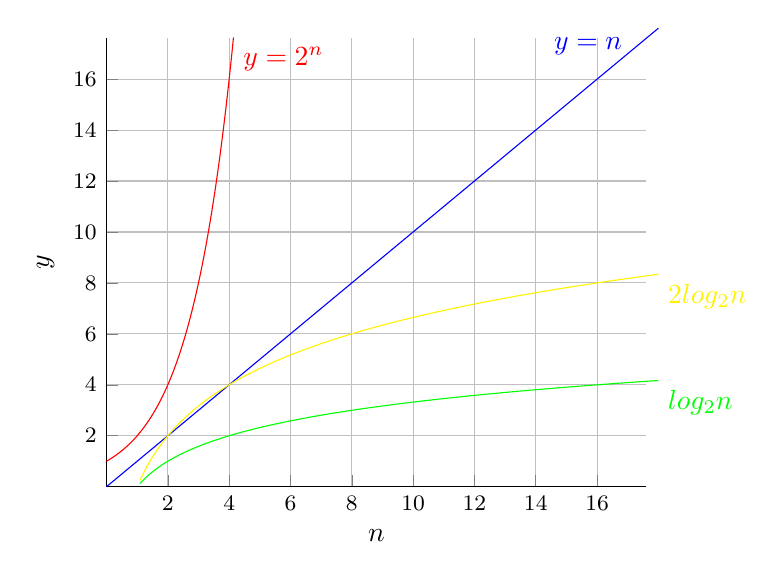
\begin{tikzpicture}[scale=1, transform shape]
\begin{axis}[grid=both,
	  xlabel=$n$,
      ylabel=$y$,
      mark = none,
      xmin = 0, ymin = 0,
      xmax = 16,ymax = 16,
      axis lines*=middle,
      enlargelimits=upper,
      clip=false,
      xtick={0,2,...,16},
      ytick={0,2,...,16}]
\addplot[red, domain=0:5,restrict y to domain=0:18, samples=100]  {pow(2,x)} node[right,anchor=north west]{$y=2^n$};
\addplot[blue, domain=0:18,restrict y to domain=0:18, samples=100]  {x} node[anchor=north east,inner xsep=3ex] {$y=n$};
\addplot[green, domain=0:18,restrict y to domain=0:18, samples=100]  {ln(x)/ln(2)} node[right,anchor=north west]{$log_2n$};
\addplot[yellow, domain=0:18,restrict y to domain=0:18, samples=100]  {2*(ln(x)/ln(2))} node[right,anchor=north west]{$2log_2n$};
\end{axis}
\end{tikzpicture}
\caption{wykres dla funkcji: $y=n$, $y=2^n$, $y=log_2n$, $y=2log_2n$}
\end{figure}

Dzieje się tak ze względu na to, że działanie algorytmów zależy od kolejności elementów w tablicy wejściowej, a nie od ich konkretnej wartości. W przypadku średnim, procedura tworzy mieszankę "dobrych" i "złych" podziałów.

\section{Najgorszy przypadek}
Istnieje też druga strona medalu i przypadek najgorszy. Następuje on, gdy podziały są maksymalnie niezrównoważone i za każdym razem tablica jest dzielona na dwie podtablice zawierające odpowiednio $n-1$ oraz 0 elementów. Wtedy koszt jednego podziału wynosi $\theta (n)$. Opisuje to rekurencyjne równanie:
\begin{equation*}
T(n) = T(n-1) + T(0) + \theta(n) = T(n-1) + \theta(n)
\end{equation*}

gdzie:

\begin{equation*}
T(n-1)
\end{equation*}

to czas przejścia po tablicy z $n-1$ elementami, $T(0)$ to czas przejścia po tablicy z 0 elementami, a $\theta(n)$ to koszt podziału najbardziej niezrównoważonego, wtedy:
\begin{equation*}
T(n-1) + \theta(n) = \theta(n^2)
\end{equation*}
Co daje czas działania tak wolny jak sortowanie przez wstawianie.

\section{Testy}
\subsection{Zależność czasu od długości listy wsadowej}
Pierwszym testem jest porównanie szybkości działania algorytmu w zależności od długości listy. Testowi poddawane są wszystkie cztery funkcje wyboru \textit{pivota}, każda funkcja w jednej iteracji otrzymuje identyczną listę określonej długości, co pozwoli na otrzymanie wiarygodnego i zdatnego do porównania wyniku:

\begin{figure}[h!]
\centering
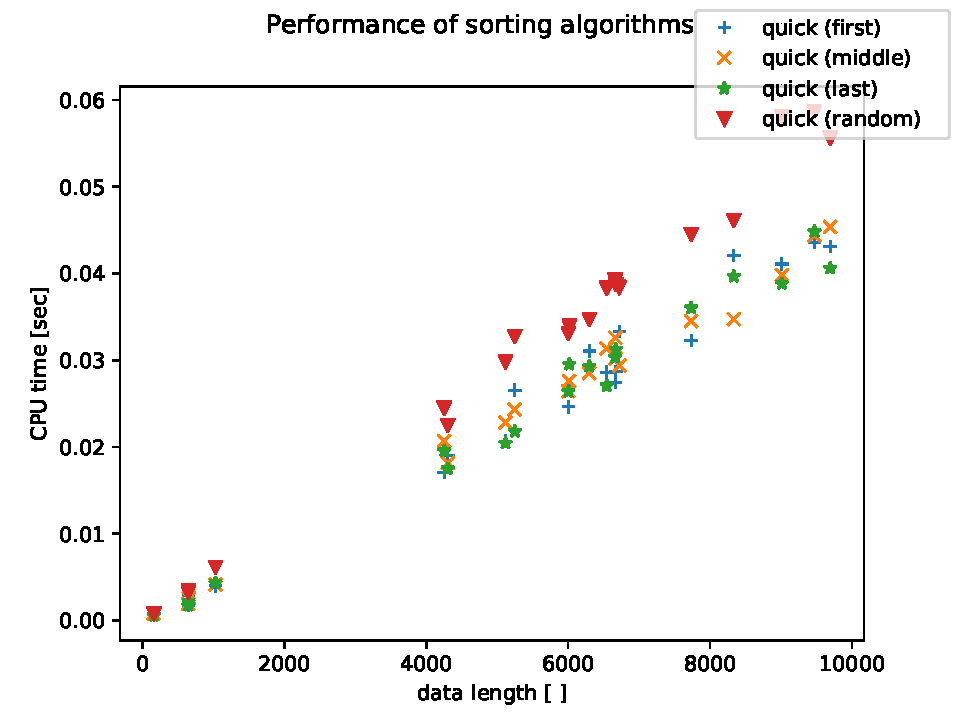
\includegraphics[scale=0.8]{Figure_1.pdf}
\caption{Wykres zależności czasu od długości listy wsadowej}
\end{figure}

\subsubsection{Wniosek}
Jest następujący: funkcja wyboru \textit{random} działa najbardziej optymalnie w każdym przypadku długości. Spowodowane jest to zjawiskiem losowego wyboru \textit{pivot'a} - daje to zawsze taką samą szansę wybrania wyniku będącego jak najbliższym wartości środkowej. 


\subsubsection{Lista w pewnym stopniu posortowana}
Rozważmy przypadek, gdy do algorytmu podawana jest lista w pewnym stopniu posortowana. Wtedy, żeby \textit{pivot} osiągnął wartość jak najbliższą wartości mediany (wtedy algorytm działa najszybciej) najrozsądniejszym wyborem \textit{pivot'a} będzie wybór losowy, gdyż szanse na wybranie każdego elementu będą identyczne.


W przypadku wyboru \textit{pivot'a} jako pierwszego lub ostatniego elementu, dla listy posortowanej w pewnym stopniu, za każdym razem istnieje ryzyko wielokrotnego wybrania mało optymalnego elementu (tj. tworzącego jeden podzbiór ze wszystkimi elementami i drugi podzbiór pusty). Powoduje to zmniejszenie efektywności algorytmu. Problem ten nie pojawi się w przypadku funkcji \textit{random}.

\subsection{Szybkość sortowania w 100 losowych przypadkach}


\textit{Rys. 2.3} przedstawia czas działania czterech sposobów wyboru \textit{pivot'a} dla stu przypadków, w przypadku gdy lista jest losowa, a długość listy jest taka sama w każdym przypadku. Można zauważyć, że w takim wypadku losowy wybór \textit{pivot'a} zazwyczaj charakteryzuje się najdłuższym czasem działania. Czerwone trójkąty na wykresie mają reprezentują zazwyczaj największą wartość, ponieważ randomizowanie wyboru powoduje dodatkową stratę czasu. Wśród pozostałych sposobów można wyróżnić tendencję dla zazwyczaj wyższych wyników przy wyborze \textit{middle} oraz mniej więcej równomierny rozkład dla \textit{last} i \textit{first}, co potwierdza wniosek, że przy losowej liście najbardziej optymalnym sposobem jest wybór pierwszego/ostatniego elementu jako \textit{pivot'a}.

\begin{figure}[h!]
\centering
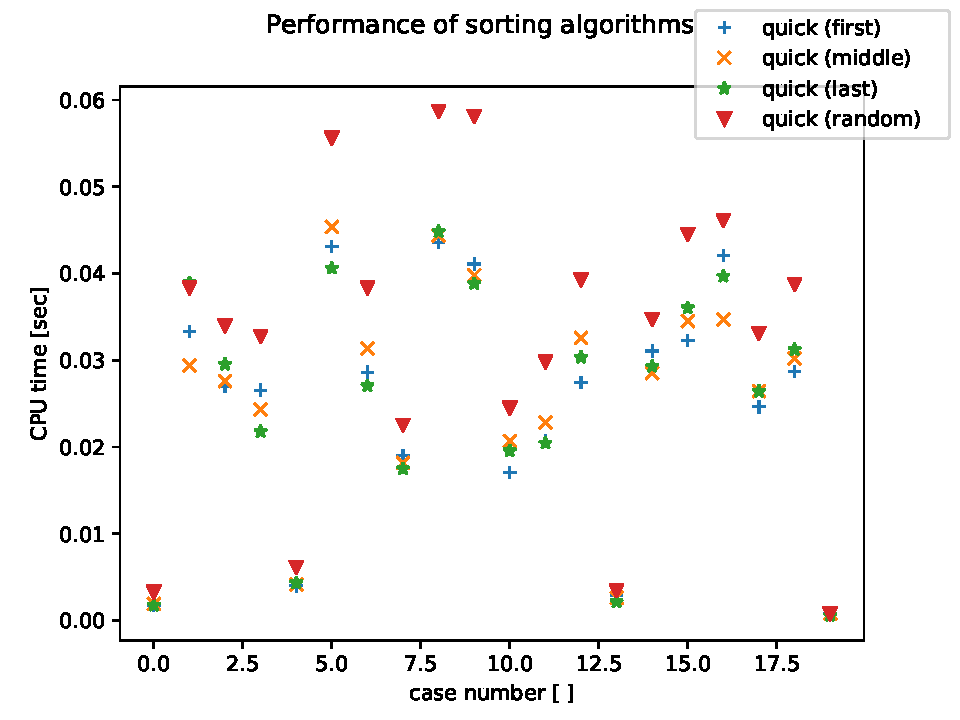
\includegraphics[scale=0.8]{Figure_2.pdf}
\caption{Wykres zależności czasu od ilości iteracji}
\end{figure}

Podsumowując, wyboru pivota powinien być uzależniony od typu danych, który jest przekazywany do algorytmu. Gdy oczekiwana struktura danych jest całkowicie nieuporządkowana, należy rozważyć randomizowaną wersję algorytmu; gdy jednak istnieją podejrzenia, że dane mogą być pewnym stopniu uporządkowane, lepszym wyborem będzie wybór pivot'a jako element ostatni, pierwszy lub środkowy.


Wyboru algorytmu sortującego powinien być uzależniony od rodzaju przekazanych danych, ponieważ istnieją algorytmy , które lepszy czas wykażą dla danych uporządkowanych (sortowanie bąbelkowe, sortowanie przez wstawianie) oraz takie, które lepiej będą się sprawdzały dla danych, które nie są uporządkowane (sortowanie przez kopcowanie, quicksort, sortowanie przez scalanie).

\nocite{*}
\bibliographystyle{plain}
\bibliography{refer.bib}
\end{document}
